\documentclass{bioinfo}
\copyrightyear{2017} \pubyear{2017}

\access{Advance Access Publication Date: Day Month Year}
\appnotes{Review article}
\graphicspath{{../figures/}}

\newcommand{\comment}[1]{\textcolor{red}{#1}}
\newcommand{\todo}[1]{\colorbox{yellow}{\parbox{1\linewidth}{#1}}}

\begin{document}
\firstpage{1}

\subtitle{Review}

\title[short Title]{Cardioinformatics: the unmet need to pioneer an emerging field at the nexus of bioinformatics and cardiology}
\author[Sample \textit{et~al}.]{Bohdan B. Khomtchouk\,$^{\text{\sfb 1,}*}$, Diem-Trang Tran\,$^{\text{\sfb 2}}$, Themistocles L. Assimes\,$^{\text{\sfb 3, 4}}$ and Or Gozani\,$^{\text{\sfb 1}}$}
\address{$^{\text{\sf 1}}$Department of Biology, Stanford University, Stanford, CA, USA \\
$^{\text{\sf 2}}$School of Computing, University of Utah, Salt Lake City, UT, USA \\
$^{\text{\sf 3}}$Department of Medicine, Division of Cardiovascular Medicine, Stanford University, Stanford, CA, USA \\
$^{\text{\sf 4}}$VA Palo Alto Health Care System, Palo Alto, CA, USA
}

\corresp{$^\ast$To whom correspondence should be addressed.}

\history{Received on XXXXX; revised on XXXXX; accepted on XXXXX}

\editor{Associate Editor: XXXXXXX}

\abstract{\textbf{Motivation:} Text Text Text Text Text Text Text Text Text Text Text Text Text
Text Text Text Text Text Text Text Text Text Text Text Text Text Text Text Text Text Text Text
Text Text Text Text Text Text Text Text Text Text Text Text Text Text Text Text Text Text Text
Text Text Text Text Text Text
Text Text Text Text Text.\\
\textbf{Results:} Text  Text Text Text Text Text Text Text Text Text  Text Text Text Text Text
Text Text Text Text Text Text Text Text Text Text Text Text Text  Text Text Text Text Text Text\\
\textbf{Availability:} Text  Text Text Text Text Text Text Text Text Text  Text Text Text Text
Text Text Text Text Text Text Text Text Text Text Text Text Text Text  Text\\
\textbf{Contact:} \href{bohdan@stanford.edu}{bohdan@stanford.edu}\\
\textbf{Supplementary information:} Supplementary data are available at \textit{Briefings in Bioinformatics}
online.}

\maketitle

\section{The current status of bioinformatics in cardiovascular disease research}
\begin{figure}
	\centering
	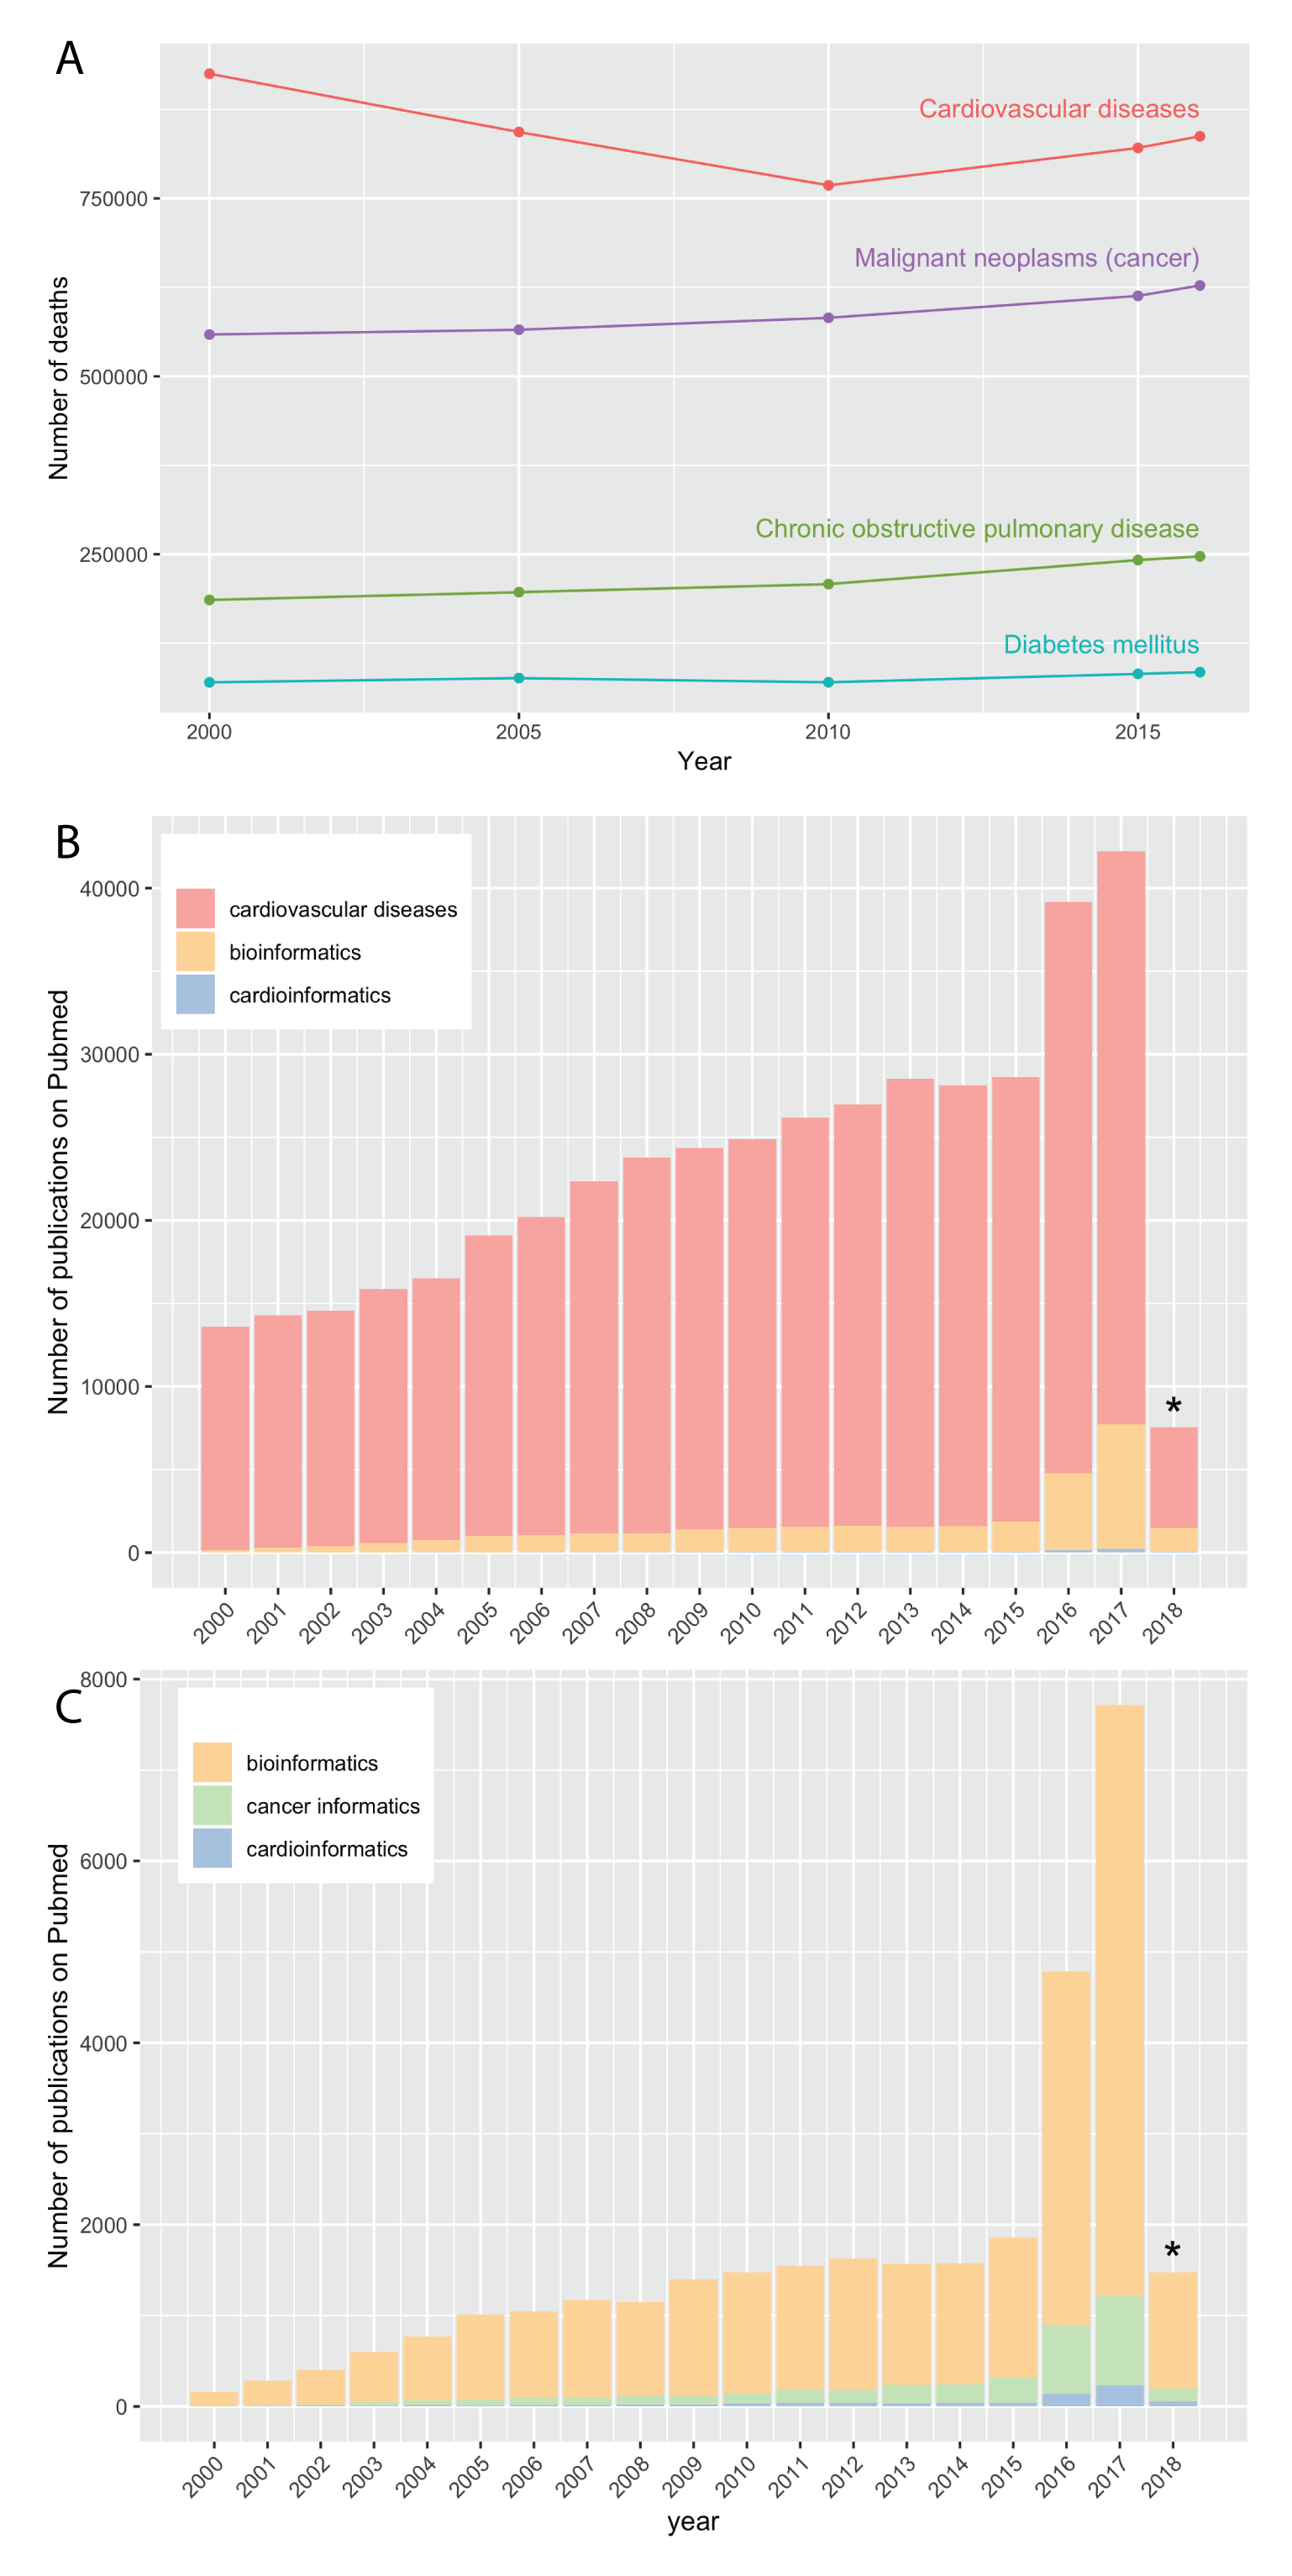
\includegraphics[width=1\linewidth]{figure1}
	\caption{\textbf{A}. Number of deaths by Non-Communicable Diseases in the US. \textbf{B}. \textbf{C}.}
	\label{fig:figure1}
\end{figure}

Cardiovascular diseases (CVD) have been persistently the leading cause of deaths by non-communicable diseases in the US for the last two decades (Figure \ref{fig:figure1}A). CVD research has steadily increased since 2000, resulting in an immense body of publications indexed in PubMed. In 2017 alone, there are more than 40000 articles classified with the subject heading "cardiovascular disease" (defined according to the Medical Subject Heading -- MeSH terms), not including reviews. (The MeSH Database entry for \textit{cardiovascular disease} includes many types of cardiovascular abnormalities which may occur in organs other than the circulatory system.) Among these outputs, the share of bioinformatics research remains modest, almost invisible. Such modest contribution of bioinformatics in cardiology is in stark contrast to that in cancer, to some extent suggesting that there are ample opportunities for cardioinformatics. In this review, we demonstrate the need of more bioinformatics studies, introduce the bountiful resources available and propose the ways to advance this field and leverage cardiovascular research.

The first draft of the human genome project had brought a lot of hope and excitement about potential advancements in the diagnosis and treatment of cardiac diseases, such as the ability to identify disease genes within the associated loci, to improve risk estimation based on more precise genotypes, or to personalize the prediction of drug effect on a patient, \citep{Komajda:2001:heart}.

%{https://www.ncbi.nlm.nih.gov/mesh/68002318} 


\section{Complexity of CVD}

\todo{Elaborate on these aspects: polygenic diseases, missing heritability, gene-environment interactions, etc. Some may be overlapping.}

%Some quantity showing the associations of CVD with genes...
%
Text Text Text Text Text Text  Text TextText Text Text Text Text Text  Text TextText Text Text Text Text Text  Text TextText Text Text Text Text Text  Text TextText Text Text Text Text Text  Text Text Text Text Text Text Text Text  Text Text Text Text Text Text Text Text  Text Text Text Text Text Text Text Text  Text Text Text Text Text Text Text Text  Text Text Text Text Text Text Text Text  Text Text Text Text Text Text Text Text  Text Text Text Text Text Text Text Text  Text Text Text Text Text Text Text Text  Text Text Text Text Text Text Text Text  Text Text Text Text Text Text Text Text  Text Text Text Text Text Text Text Text  Text Text Text Text Text Text Text Text  Text Text Text Text Text Text Text Text  Text Text Text Text Text Text Text Text  Text Text Text Text Text Text Text Text  Text Text Text Text Text Text Text Text  Text Text Text Text Text Text Text Text  Text Text Text Text Text Text Text Text  Text Text Text Text Text Text Text Text  Text Text Text Text Text Text Text Text  Text Text Text Text Text Text Text Text  Text Text Text Text Text Text Text Text  Text Text Text Text Text Text Text Text  Text Text Text Text Text Text Text Text  Text Text Text Text Text Text Text Text  Text Text Text Text Text Text Text Text  Text Text Text Text Text Text Text Text  Text Text Text Text Text Text Text Text  Text Text Text Text Text Text Text Text  Text Text Text Text Text Text Text Text  Text Text Text Text Text Text Text Text  Text Text Text Text Text Text Text Text  Text Text Text Text Text Text Text Text  Text Text Text Text Text Text Text Text  Text Text Text Text Text Text Text Text  Text Text Text Text Text Text Text Text  Text Text Text Text Text Text Text Text  Text Text Text Text Text Text Text Text  Text Text Text Text Text Text Text Text  Text Text Text Text Text Text Text Text  Text Text Text Text Text Text Text Text  Text Text Text Text Text Text Text Text  Text Text Text Text Text Text Text Text  Text Text Text Text Text Text Text Text  Text Text Text Text Text Text Text Text  Text Text Text Text Text Text Text Text  Text Text Text Text Text Text Text Text  Text Text Text Text Text Text Text Text  Text Text Text Text Text Text Text Text  Text Text Text Text Text Text Text Text  Text Text Text Text Text Text Text Text  Text Text Text Text Text Text Text Text  Text Text Text Text Text Text Text Text  Text Text Text Text Text Text Text Text  Text Text Text Text Text Text Text Text  Text Text Text Text Text Text Text Text  Text Text Text Text Text Text Text Text  Text Text Text Text Text Text Text Text  Text Text Text Text Text Text Text Text  Text Text Text Text Text Text Text Text  Text Text Text Text Text Text Text Text  Text Text Text Text Text Text Text Text  Text Text Text Text Text Text Text Text  Text Text Text Text Text Text Text Text  Text Text  

\section{Profusion of data}

Technological advances brought about the accumulation of biological data, both in the number of data points, and the number of dimensions in each data point.
High-throughput profiling techniques are inarguably the main drive in creating high-dimensional data (DNA, RNA, protein levels).
A glimpse into central repositories such as GEO or dbGaP hinted at the amount of data points that can be accumulated from small  studies. Depending on the questions at hands, the precise definition of a data point can vary. In most cases, it can be equivalent to the number biological samples or that of individual donors. Although studies directly related to CVDs are of interest when it comes to future CVD research, a significant number of data points from non-CVD studies can be put into use, for example, when these studies investigated samples of cardiovascular origin (heart or vascular tissues).

\begin{figure}[!tpb]%figure1
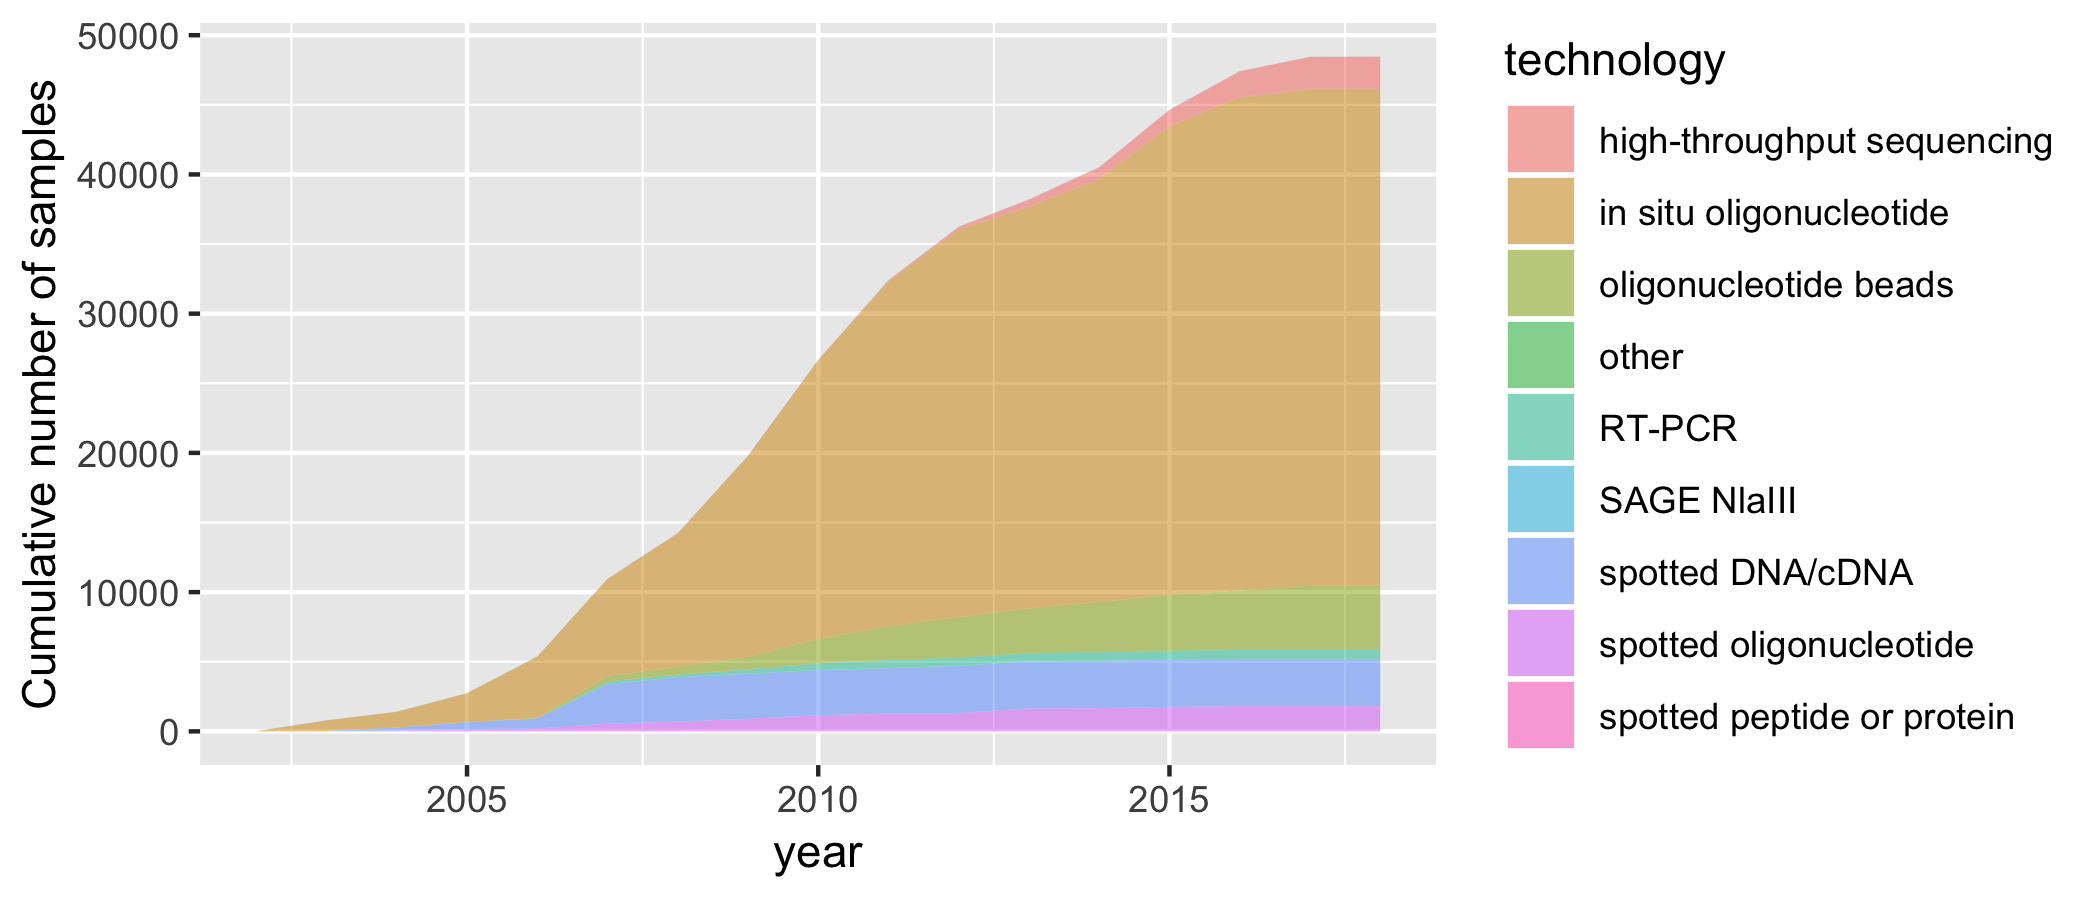
\includegraphics[width=1\linewidth]{gsm_count_by_tech.png}
	\caption{The cumulative number of samples deposited on GEO.}\label{fig:01}
\end{figure}

\begin{table}[!t]
	\processtable{Number of samples available on GEO that are of potential use of cardioinformatics research, including those deposited by CVD studies and non-CVD studies.\label{tab:geoSamples}} {\begin{tabular}{@{}llll@{}}\toprule 
			molecule &non-CVD studies & CVD studies \\ \midrule
			genomic DNA &            440 &        8525  \\
			polyA RNA &             89 &         392  \\
			total RNA &           2974 &       39540  \\
			other &             NA &           5  \\
			protein &             NA &           3  \\ \botrule
	\end{tabular}}{This is a footnote}
\end{table}

The figures given in Table \ref{tab:dbgapSubject} are in fact conservative estimates of the data generated so far among the research community. A much larger amount of data are stored on dbGaP and accessible upon approval of data request. Among these, the number of subjects involved in CVD research alone are more than 600000. %658305 to be exact

\todo{supplement table if necessary}

Text Text Text Text Text Text  Text Text Text Text Text Text Text Text  Text Text Text Text Text Text Text Text  Text Text Text Text Text Text Text Text  Text Text Text Text Text Text Text Text  Text Text Text Text Text Text Text Text  Text Text Text Text Text Text Text Text  Text Text Text Text Text Text Text Text  Text Text Text Text Text Text Text Text  Text Text Text Text Text Text Text Text  Text Text Text Text Text Text Text Text  Text Text Text Text Text Text Text Text  Text Text Text Text Text Text Text Text  Text Text Text Text Text Text Text Text  Text Text Text Text Text Text Text Text  Text Text Text Text Text Text Text Text  Text Text Text Text Text Text Text Text  Text Text Text Text Text Text Text Text  Text Text Text Text Text Text Text Text  Text Text Text Text Text Text Text Text  Text Text Text Text Text Text Text Text  Text Text Text Text Text Text Text Text  Text Text Text Text Text Text Text Text  Text Text 
% Please add the following required packages to your document preamble:
% \usepackage{booktabs}
\begin{table}[]
	\caption{The subject count aggregated from studies deposited in dbGaP, licensed for General Research Use}
	\label{tab:dbgapSubject}
	\begin{tabular}{l l l}
		\toprule
		& \textbf{CVD} &  \textbf{All}                         \\ \midrule
		16s rRNA (NGS)                 &     0 &      92 \\
		CNV Genotypes                  &     0 &   48972 \\
		Chromatin (NGS)                &     0 &     139 \\
		Genomic Sequence Amplicon (NGS)&     0 &       8 \\
		Methylation (CpG)              &     0 &     657 \\
		Methylome sequencing           &     0 &     152 \\
		QTL Results                    &     0 &     281 \\
		RNA Seq (NGS)                  &   333 &    1498 \\
		SNP Genotypes (Array)          &  6658 &  113597 \\
		SNP Genotypes (NGS)            &  4277 &   11786 \\
		SNP Genotypes (PCR)            &     0 &      10 \\
		SNP Genotypes (imputed)        &     0 &   29693 \\
		SNP/CNV Genotypes (NGS)        &     0 &     936 \\
		SNP/CNV Genotypes (imputed)    &     0 &    9291 \\
		SNV (.MAF)                     &     0 &       2 \\
		SNV Aggregate (.MAF)           &     0 &     570 \\
		Targeted Genome (NGS)          &     0 &    9918 \\
		Whole Exome (NGS)              &  5518 &   12771 \\
		Whole Genome (NGS)             &     0 &    1245 \\
		mRNA Expression (Array)        &     0 &     798 \\
		miRNA (NGS)                        & 0 &   228 \\ \hline
	\end{tabular}
\end{table}

Text Text Text Text Text Text  Text Text Text Text Text Text Text Text  Text Text Text Text Text Text Text Text  Text Text Text Text Text Text Text Text  Text Text Text Text Text Text Text Text  Text Text Text Text Text Text Text Text  Text Text Text Text Text Text Text Text  Text Text Text Text Text Text Text Text  Text Text Text Text Text Text Text Text  Text Text Text Text Text Text Text Text  Text Text Text Text Text Text Text Text  Text Text Text Text Text Text Text Text  Text Text Text Text Text Text Text Text  Text Text Text Text Text Text Text Text  Text Text Text Text Text Text Text Text  Text Text Text Text Text Text Text Text  Text Text Text Text Text Text Text Text  Text Text Text Text Text Text Text Text  Text Text Text Text Text Text Text Text  Text Text Text Text Text Text Text Text  Text Text Text Text Text Text Text Text  Text Text Text Text Text Text Text Text  Text Text Text Text Text Text Text Text  Text Text 
%
\section{Solutions from bioinformatics}
%%
\subsection{The multi-layered paths from genome to phenotype}

Text Text Text Text Text Text  Text Text Text Text Text Text Text Text  Text Text Text Text Text Text Text Text  Text Text Text Text Text Text Text Text  Text Text Text Text Text Text Text Text  Text Text Text Text Text Text Text Text  Text Text Text Text Text Text Text Text  Text Text Text Text Text Text Text Text  Text Text Text Text Text Text Text Text  Text Text Text Text Text Text Text Text  Text Text Text Text Text Text Text Text  Text Text Text Text Text Text Text Text  Text Text Text Text Text Text Text Text  Text Text Text Text Text Text Text Text  Text Text Text Text Text Text Text Text  Text Text Text Text Text Text Text Text  Text Text Text Text Text Text Text Text  Text Text Text Text Text Text Text Text  Text Text Text Text Text Text Text Text  Text Text Text Text Text Text Text Text  Text Text Text Text Text Text Text Text  Text Text Text Text Text Text Text Text  Text Text Text Text Text Text Text Text  Text Text Text Text Text Text Text Text  Text Text Text Text Text Text Text Text  Text Text Text Text Text Text Text Text  Text Text Text Text Text Text Text Text  Text Text Text Text Text Text Text Text  Text Text Text Text Text Text Text Text  Text Text Text Text Text Text Text Text  Text Text Text Text Text Text Text Text  Text Text Text Text Text Text Text Text  Text Text Text Text Text Text Text Text  Text Text Text Text Text Text Text Text  Text Text Text Text Text Text Text Text  Text Text Text Text Text Text Text Text  Text Text Text Text Text Text Text Text  Text Text Text Text Text Text Text Text  Text Text Text Text Text Text Text Text  Text Text 
%
\todo{Tentative: A figure/table enlisting layers of modifications that contribute to determine a phenotype, with the corresponding experimental techniques}
%%
%\begin{itemize}
%	\item genome
%	\item epigenome
%	\item transcriptome: mRNA, non-coding RNA: microRNA, long non-coding RNA
%	\item 	proteome
%	\item	metabolome
%\end{itemize}
%%environmental factors
%
%
\subsection{Bioinformatics as a tool-kit}

As early as 1999 when complete genome sequencing and high-throughput transcriptomic profiling are on the horizon, research community have started to recognize the critical use of bioinformatics analyses in generating insights from these data \citep{Claverie:1999:Computational}.
The infrastructure for bioinformatics analyses now is even more mature, thanks to cloud computing \citep{Langmead:2018:Cloud}, secured data storage and management.



Text Text Text Text Text Text  Text Text Text Text Text Text Text Text  Text Text Text Text Text Text Text Text  Text Text Text Text Text Text Text Text  Text Text Text Text Text Text Text Text  Text Text Text Text Text Text Text Text  Text Text Text Text Text Text Text Text  Text Text Text Text Text Text Text Text  Text Text Text Text Text Text Text Text  Text Text Text Text Text Text Text Text  Text Text Text Text Text Text Text Text  Text Text Text Text Text Text Text Text  Text Text Text Text Text Text Text Text  Text Text Text Text Text Text Text Text  Text Text Text Text Text Text Text Text  Text Text Text Text Text Text Text Text  Text Text Text Text Text Text Text Text  Text Text Text Text Text Text Text Text  Text Text Text Text Text Text Text Text  Text Text Text Text Text Text Text Text  Text Text Text Text Text Text Text Text  Text Text Text Text Text Text Text Text  Text Text Text Text Text Text Text Text  Text Text Text Text Text Text Text Text  Text Text Text Text Text Text Text Text  Text Text Text Text Text Text Text Text  Text Text Text Text Text Text Text Text  Text Text Text Text Text Text Text Text  Text Text Text Text Text Text Text Text  Text Text Text Text Text Text Text Text  Text Text Text Text Text Text Text Text  Text Text Text Text Text Text Text Text  Text Text Text Text Text Text Text Text  Text Text Text Text Text Text Text Text  Text Text Text Text Text Text Text Text  Text Text Text Text Text Text Text Text  Text Text Text Text Text Text Text Text  Text Text Text Text Text Text Text Text  Text Text Text Text Text Text Text Text  Text Text 
%
%\subsubsection{Basic research}
%for data management, computational analysis, visual representation, etc.
%
%\subsubsection{Clinical application}
%
%
\subsection{Bioinformatics as a perspective}

Bioinformatics is more than a powerful toolkit to manipulate the large amount of data beyond human capability. The paradigm shift from the single physical gene to the "eigengenes" in studying complex diseases \citep{Weiss:2012:Good} is a pragmatic approach.


Text Text Text Text Text Text  Text Text Text Text Text Text Text Text  Text Text Text Text Text Text Text Text  Text Text Text Text Text Text Text Text  Text Text Text Text Text Text Text Text  Text Text Text Text Text Text Text Text  Text Text Text Text Text Text Text Text  Text Text Text Text Text Text Text Text  Text Text Text Text Text Text Text Text  Text Text Text Text Text Text Text Text  Text Text Text Text Text Text Text Text  Text Text Text Text Text Text Text Text  Text Text Text Text Text Text Text Text  Text Text Text Text Text Text Text Text  Text Text Text Text Text Text Text Text  Text Text Text Text Text Text Text Text  Text Text Text Text Text Text Text Text  Text Text Text Text Text Text Text Text  Text Text Text Text Text Text Text Text  Text Text Text Text Text Text Text Text  Text Text Text Text Text Text Text Text  Text Text Text Text Text Text Text Text  Text Text Text Text Text Text Text Text  Text Text Text Text Text Text Text Text  Text Text Text Text Text Text Text Text  Text Text Text Text Text Text Text Text  Text Text Text Text Text Text Text Text  Text Text Text Text Text Text Text Text  Text Text Text Text Text Text Text Text  Text Text Text Text Text Text Text Text  Text Text Text Text Text Text Text Text  Text Text Text Text Text Text Text Text  Text Text Text Text Text Text Text Text  Text Text Text Text Text Text Text Text  Text Text Text Text Text Text Text Text  Text Text Text Text Text Text Text Text  Text Text Text Text Text Text Text Text  Text Text Text Text Text Text Text Text  Text Text Text Text Text Text Text Text  Text Text 
%

\enlargethispage{12pt}




\section*{Acknowledgements}

Text Text Text Text Text Text  Text Text.  
\vspace*{-12pt}

\section*{Funding}

This work has been supported by the... Text Text  Text Text.\vspace*{-12pt}

\bibliographystyle{natbib}
%\bibliographystyle{achemnat}
%\bibliographystyle{plainnat}
%\bibliographystyle{abbrv}
%
%\bibliographystyle{plain}
%
\bibliography{cardio}



\end{document}
